\hoofdstuk{Preliminary research}

The goal of the preliminary research is to determine whether or not an existing solution offers cross-platform mobile application development as defined by Lunatechs' criteria.
%todo: And whether or not it's better to devise my own custom solution...

\paragraaf{Introduction}
In todays industry there exist several cross-platform mobile application development frameworks which offer a solution to cross-platform problem. All of these frameworks provide a solution for crossing the bridge between platforms. In order to determine which framework could be adopted by Lunatech for mobile development the following criteria have been determined for comparison:

\begin{enumerate}
\item \emph{Platform support}\\
Which platforms and their versions are supported by the framework.
\item \emph{Native UI support}\\
Whether or not native user interface elements are supported for each supported platform.
\end{enumerate}
\noindent secondary criteria:
\begin{enumerate}
\item \emph{Programming language}\\
Which programming language is used to develop using the framework.
\item \emph{IDE} (Integrated Development Environment)\\
Which IDE can be used to develop using with the framework.
\item \emph{License type}\\
Which license types are available.
\item \emph{Application type}\\
Which type of mobile application is produced using this framework.
\end{enumerate}

The cross-platform criterium is based on Lunatechs requirement to build mobile applications for the operating systems have at least a 10 percent market share in the European continent. Second comes the support for native user interface elements. Together these criteria form the essence of the main research question: \emph{"How to develop a cross-platform mobile application while retaining the native look-and-feel?"}
The remaining criteria are of secondary importance, they will provide more detailed means to compare the frameworks which offer native user interface support.

Based on the previous statement and criteria a hypothesis can be formed:
\begin{shadequote}
There is an existing solution which offers cross-platform mobile application development as defined by Lunatechs' criteria.\par\emph{W. de Kraker, 2012}
\end{shadequote}


%\subparagraaf{Framework requirements}
%
%A cross-platform mobile application development framework has to:
%\begin{itemize}
%\item Support cross-platform mobile application development.\\
%Build an application which runs on multiple platforms, originating from a single codebase.
%\item Supported platforms should be at minimum iOS and Android.\\
%As decided in Chapter Defining the context, section \emph{Mobile platforms}
%\item Be able to offer the native look-and-feel.\\
%As defined in Chapter Defining the context, section \emph{Defining native}
%\end{itemize}


\paragraaf{Method}
%todo, in this paragraph...
% listing van bestaande frameworks.
% toepassen criterea.
% testwijze (benchmak app)
% beste kiezen om mee verder te gaan
In order to test the hypothesis it is necessary to conduct a market survey to determine which solutions to cross-platform app development are available on todays market and which of those meet the criteria. Each solution will be evaluated during a test in which a benchmark application will be developed using the solution. The resulting evaluations will be compared. The solution which offers the most complete set of features will be deemed potentially viable for commercial use by Lunatech. 

\begin{centering}
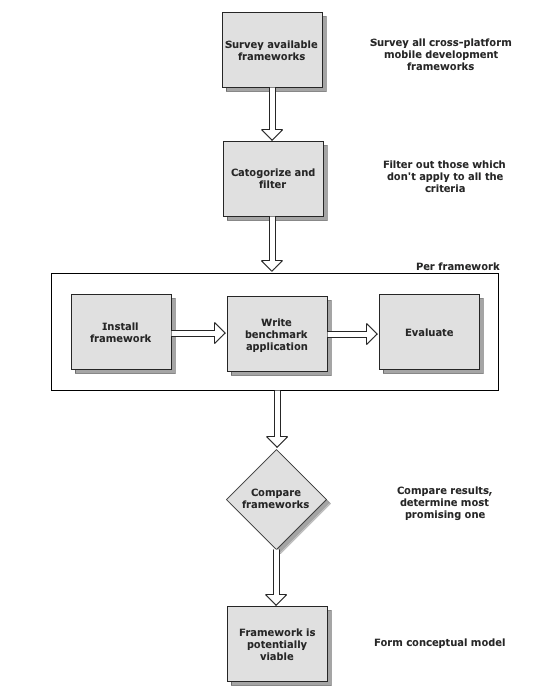
\includegraphics[scale=0.3]{images/preliminary}\\{Preliminary research structure}\\
\end{centering}
\subparagraaf{Selection}

There are over 30 frameworks which offer cross-platform development of mobile applications\cite{Wikipedia2012}. These frameworks have been added to an initial list.\footnote{see appendix: \emph{Existing solutions}} This initial list contains only frameworks which adhere to the requirement of supporting cross-platform mobile application development. The frameworks in the list are categorized by the first set of criteria.

To determine which frameworks should be included in the comparison we'll take a closer look at each and filter out those who don't adhere to criteria of supporting native user elements. This should leave us with an acceptable number of frameworks to compare. Acceptable in this scenario will be 5. Which is the goal because the timeframe of the internship doesn't allow for more.



\subparagraaf{Benchmark app}
In order to evaluate each framework I've decided to build a application with all of them. The application will have the same requirements on each platform. Before the evaluation process begins i'll write the application first on a native platform, the results of building it natively will serve as benchmark setting during the evaluation, hence the term: \emph{benchmark app}

The application should be related to what Lunatech might anticipate for mobile contracts. In this case the use case was taken from \emph{Stager}. Stager is a modern web-based resource planning and ticketing application to help manage live music events. Lunatech took the opportunity to use the relatively new Play framework to build a web application with an HTML5 and Java architecture. The application should be a publicity app, allowing for users to view published events and share them on social media.

This concludes that the app should be able to:
\begin{itemize}
	\item display events from the xml based atom feed,
	\item show event details,
	\item allow for sharing of events to social media
\end{itemize}
The design will be based on the website of an live music venue which already uses Stager to publish their events. WORM.ORG

%requirement specs. feed/xpath/sharekit/ui tools
For the native version of the benchmark application I've chosen to use the iOS platform simply for practical reasons, because I have an iOS device in my direct availability for testing.

It took 3 days to complete the benchmark app, from which the majority of the time was spend on parsing data using x-path, which I had never used before.
\begin{figure}%
	\centering
	\parbox{0.0in}
	\qquad
	\begin{minipage}{2.2in}%
		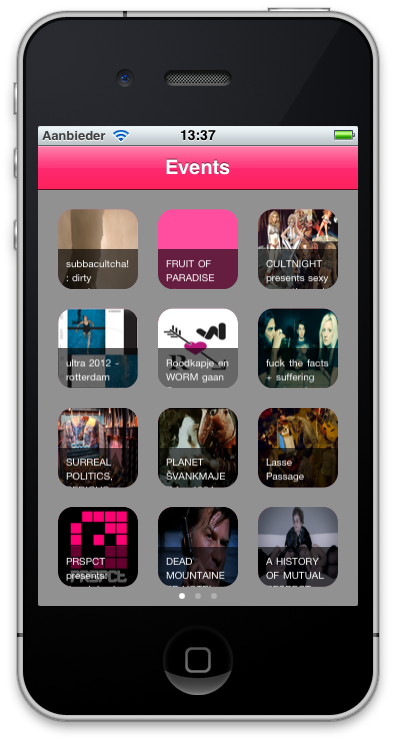
\includegraphics[scale=0.15]{images/benchmarkapp01.png}
		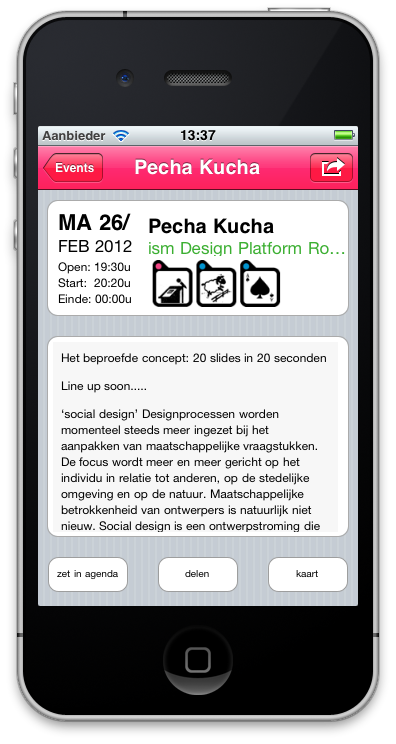
\includegraphics[scale=0.15]{images/benchmarkapp02.png}
	\end{minipage}%
	\caption{iOS version of the benchmark application}%
	\label{fig:1figs}%
\end{figure}



\subparagraaf{Evaluation process}
Estimated is that it takes 4 days to do experiments with a framework, this is based on N+1 in which N is the number of days it took to develop the benchmark app + 1 to familiarize with the framework. If in those 4 days I'm unable to complete the benchmark app, it is still a result. The experiment consumes a timespan of 32 hours per framework and consist of the following activities:

\begin{itemize}
	\item Install framework
	\item Familiarize with how it works
	\item Rewrite the benchmark app in it
	\item Noting down results and documenting the experience
\end{itemize}

The remaining framework will be Evaluated on available of documentation, licensing, community, and flexibility.

\paragraaf{Results}
Work in progress
This paragraph will summarize the results of the research, more details of the results are included as a appendices (list + evaluations) (todo)%todo referal. #TODO

From 30 existing solutions a total of 4 frameworks were selected to be evaluated:
\begin{itemize}
	\item Titanium
	\item RhoMobile
	\item MoSync
	\item Worklight
\end{itemize} 



{\bf Titanium}, the first framework put under evaluation. In the 3 days available for rewriting the benchmark app only the first two features were implemented successfully.

However there was a complication: Titanium does not support the DOM3 specifications. Not having been developed beyond DOM2 specifications the required methods to evaluate an XML document where missing, to be more precise, x-path could not be used. This is particularly troublesome because the resulting solution required hardcoded namespace resolving, which is against best practice. %forced to write some ugly parsing functions that made me want to rm -rf my disk. But it worked. %DONE? herzien.

Overall developing with Titanium proceeded really well, with exception for the DOM issue. The built results were as expected: cross-platform with the native look and feel.

Second up: {\bf Rhomobile}. Up on installing it and reading the quick start guide it turns out that elements are not by definition \emph{native} but HTML elements mimicking the native user interface style. The native feature advertised on their website referred to the fact that Rhomobile can encapsulate your web app in a web-view. This essentially devaluates the application type to Web-view based hybrid application as defined in chapter \emph{Defining the context}, section \emph{Alternative mobile application types}.

After some further research it turns out Rhomobile does have \emph{some} support for native user interface elements, however only the very basic. When a the developer wants to use an element not in that list, he or she has to implement it in native code. \cite{Rhomobile2012} This does not how the cross-platform definition was envisioned by Lunatech.

{\bf MoSync} was third up. During the installation of the framework the installed prompted for the system location of \emph{PhoneGap}, it would not install without. As it turns out, the developers of MoSync sync have the same definition for native as Rhomobile. The native feature advertised on their website referred to the fact that MoSync can encapsulate your web app in a web-view. The user interface is built using a PhoneGap implementation. Further research did not show a way for building actual native user interface elements using MoSync.

Last up is {\bf Worklight}. Worklight also required PhoneGap. Even though Worklight classifies itself as producing actual native applications, it merely encapsulates a PhoneGap built user interface. The value Worklight brings is in their API which augments the PhoneGap application by exposing a JavaScript API to access some of the devices' native features.


\subparagraaf{Conclusion}
The goal of this preliminary research was to "\emph{determine whether or not an existing solution offers cross-platform mobile application development as defined by Lunatechs' criteria.}".  Surveying and categorizing the available frameworks on the market resulted in a list of 4 possible solutions. By evaluating each solution it turned out that Titanium meets the criteria set by Lunatech. Therefor the following conceptual model can be defined:
\begin{shadequote}
Titanium offers cross-platform mobile application development as defined by Lunatechs' criteria.\par\emph{W. de Kraker, 2012}
\end{shadequote}